% This file was created by matlab2tikz.
%
%The latest updates can be retrieved from
%  http://www.mathworks.com/matlabcentral/fileexchange/22022-matlab2tikz-matlab2tikz
%where you can also make suggestions and rate matlab2tikz.
%
\documentclass[tikz]{standalone}
\usepackage[T1]{fontenc}
\usepackage[utf8]{inputenc}
\usepackage{pgfplots}
\usepackage{grffile}
\pgfplotsset{compat=newest}
\usetikzlibrary{plotmarks}
\usepgfplotslibrary{patchplots}
\usepackage{amsmath}
\usetikzlibrary{decorations.markings}
\begin{document}
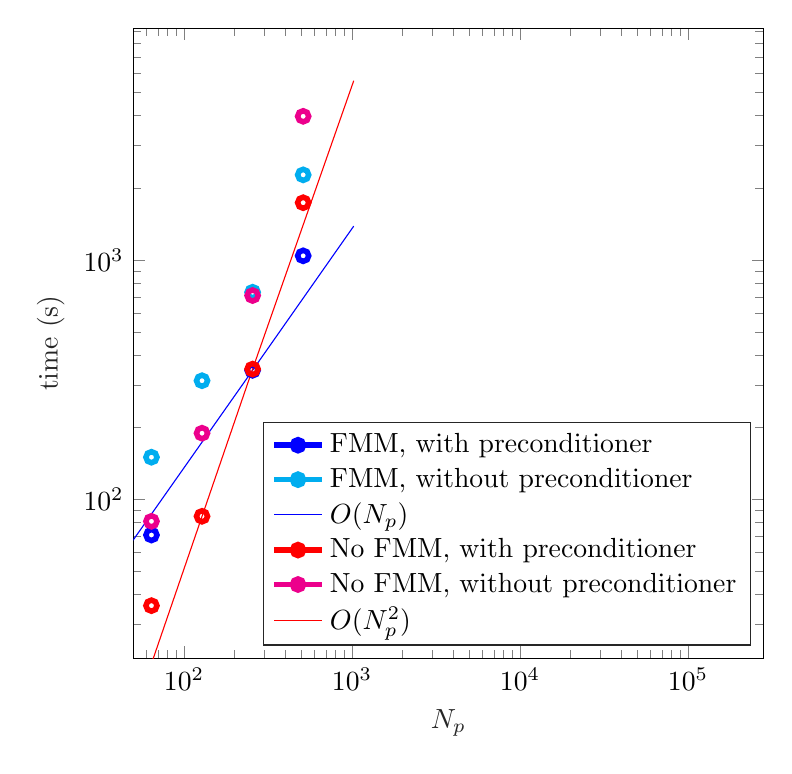
\begin{tikzpicture}

\begin{axis}[%
at={(0cm,0cm)},
width=8cm,
height=8cm,
scale only axis,
xmode=log,
xmin=50,
xminorticks=true,
xlabel style={font=\color{white!15!black}},
xlabel={$N_p$},
ymode=log,
yminorticks=true,
ylabel style={font=\color{white!15!black}},
ylabel={time (s)},
axis background/.style={fill=white},
legend style={legend cell align=left, align=left, draw=white!15!black, at={(0.98,0.02)}, anchor=south east}
]
\addplot [color=blue, line width=2.0pt, draw=none, mark=o, mark options={solid, blue}]
  table[row sep=crcr]{%
8 39\\
16 34\\
32 43\\
64 71\\
128141\\
256 346\\
512 1040\\
};
\addlegendentry{ FMM, with preconditioner}

\addplot [color=cyan, line width=2.0pt, draw=none, mark=o, mark options={solid, cyan}]
  table[row sep=crcr]{%
8 66\\
16 71\\
32 91\\
64 150\\
128 313\\
256 733\\
512 2265\\
};
\addlegendentry{ FMM, without  preconditioner}

\addplot [color=blue]
  table[row sep=crcr]{%
32 43.5\\
256 346\\
1024 1384\\
};
\addlegendentry{$O(N_p)$}

\addplot [color=red, line width=2.0pt, draw=none, mark=o, mark options={solid, red}]
  table[row sep=crcr]{%
8 15\\
16 14\\
32 20\\
64 36\\
128 85\\
256 350\\
512 1733\\
};
\addlegendentry{No FMM, with preconditioner}

\addplot [color=magenta, line width=2.0pt, draw=none, mark=o, mark options={solid, magenta}]
  table[row sep=crcr]{%
8 47\\
16 33\\
32 43\\
64 81\\
128 189\\
256 710\\
512 3978\\
};
\addlegendentry{No FMM, without preconditioner}

\addplot [color=red]
  table[row sep=crcr]{%
32 5\\
256 350\\
1024 5600\\
};
\addlegendentry{$O(N_p^2)$}

\end{axis}
\end{tikzpicture}%
\end{document}